\section{MIP}
\subsection{Decision variables}
\subsubsection{matches}
The binary decision variables $X_{wpm}$ are equal to 1 iff in week w and period p match m is played.

\subsubsection{slots}
The binary decision variables $A_{wp}$ determine which team plays at home and which away. A is indexed by weeks and periods, so $A_wp$ corresponds to the matchup between teams $t_1, t_2$ in week w and period p; if $A_{wp} = 0$ then $t_1$ plays at home and $t_2$ away, if, otherwise, $A_{wp} = 1$ the order is reversed.

\subsubsection{team periods of play}
The binary variables TP are used to constrain each team to playing at most twice in the same period. $TP_{twp} = 1$ iff team t plays in week w and period p. 

\subsubsection{home games counter}
To compute the common objective function in MIP, it is necessary to introduce an array of integer auxiliary variables H such that $H[t]$ is the number of home games team t plays, bounded in $[0, n-1]$.

\subsection{Objective variables}
To compute D as the maximum difference between games played at home and away for all teams, we first find for each team the number of games played at home (2), and then constraint D as being greater or equal than the difference of home and away games for each team, given that we have a minimization problem this is effectively equivalent to computing the max. The absolute value of the difference is not computed explicitly but decomposed into 2 inequalities (3)(4). Finally, we look for the minimum of D (1)

\begin{align}
    &\min  D \\
    H_t =& \sum_{w, p} (A_{wp} = 0 \land G_{wp}[\text{home}] = t) \notag \\
    +& \sum_{w, p} (A_{wp} = 1 \land G_{wp}[\text{away}] = t) \hspace{20px}  &&t =1, \dots, n\\
    D &\geq 2H_t - (n-1) && t = 1, \dots, n\\
    D & \geq -(2 H_t - (n-1)) && t = 1, \dots, n
\end{align}


\subsection{Constraints}
\subsubsection{periods and matches}
Due to how the decision variables are defined, it was necessary to impose that each period in each week is assigned a single match (5) and each match is assigned to a single period (6).

\begin{align}
    \sum_{m = 1}^{n/2} X_{wpm} &= 1 \hspace{20px} p =1, \dots, n/2 \hspace{10px} w = 1,\dots, n-1 \\
    \sum_{p = 1}^{n/2} X_{wpm} &= 1 \hspace{20px} m = 1, \dots, n/2 \hspace{10px} w = 1,\dots, n-1
\end{align}

\subsubsection{team playing at most twice in the same period}
The constraint on teams playing at most twice in the same period was imposed by first linking the variables of X to those in TP based on the values in G (7) and then imposing that the sum of periods of play is smaller than 2 (8). 

\begin{align}
    TP_{twp} &= X_{wpm} \hspace{20px} G_{wm} =(t1, t2) \land (t = t1 \lor t=t2) \hspace{20px} \forall t \forall p  \forall w\\
    \sum_{w=1}^{n-1} &TP_{twp} \leq 2 \hspace{40px} t=1, \dots, n \hspace{10px} p = 1, \dots, n/2
\end{align}

\subsection{Validation}
\subsubsection*{Experimental design}
The model was written in Python by making use of the PuLP library and the solvers tested on the MIP model were: CBC 2.10.3, HiGHS 1.10.0, CPLEX 22.1.1 and SCIP 5.5.0 with their default parameters. The time elapsed to find an optimal solution, within the 300 second time limit, was measured and results presented in Fig.\ref{fig:MIP-solution} . All tests were run on a single core of an Intel i7-10750H CPU.

\subsubsection*{Experimental results}
As shown in Fig. \ref{fig:MIP-solution} CBC had the worst performance, it isn't able to find the optimal solution for n greater than 14. CPLEX, instead, was the fastest up to n=14 but after n=16 it stopped finding the optimal solution. HiGHS was able to find an optimal solution up to n=18 and SCIP, the best performer of the four, was able to reach n=20.

It was also verified that the solvers either found and optimal solution or no solution at all.

\begin{figure}
    \centering
    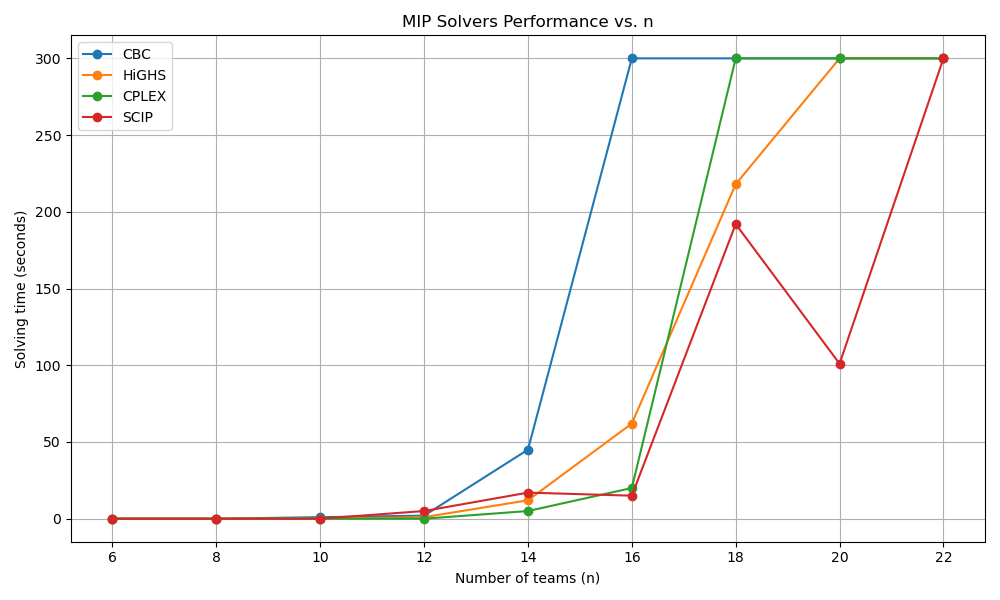
\includegraphics[width=0.8\linewidth]{img/MIP-result.png}
    \caption{MIP optimization}
    \label{fig:MIP-solution}
\end{figure}